\section{Grundglieder \skript{25ff, 202-206}}
	\subsection{statische Glieder \skript{28}}
		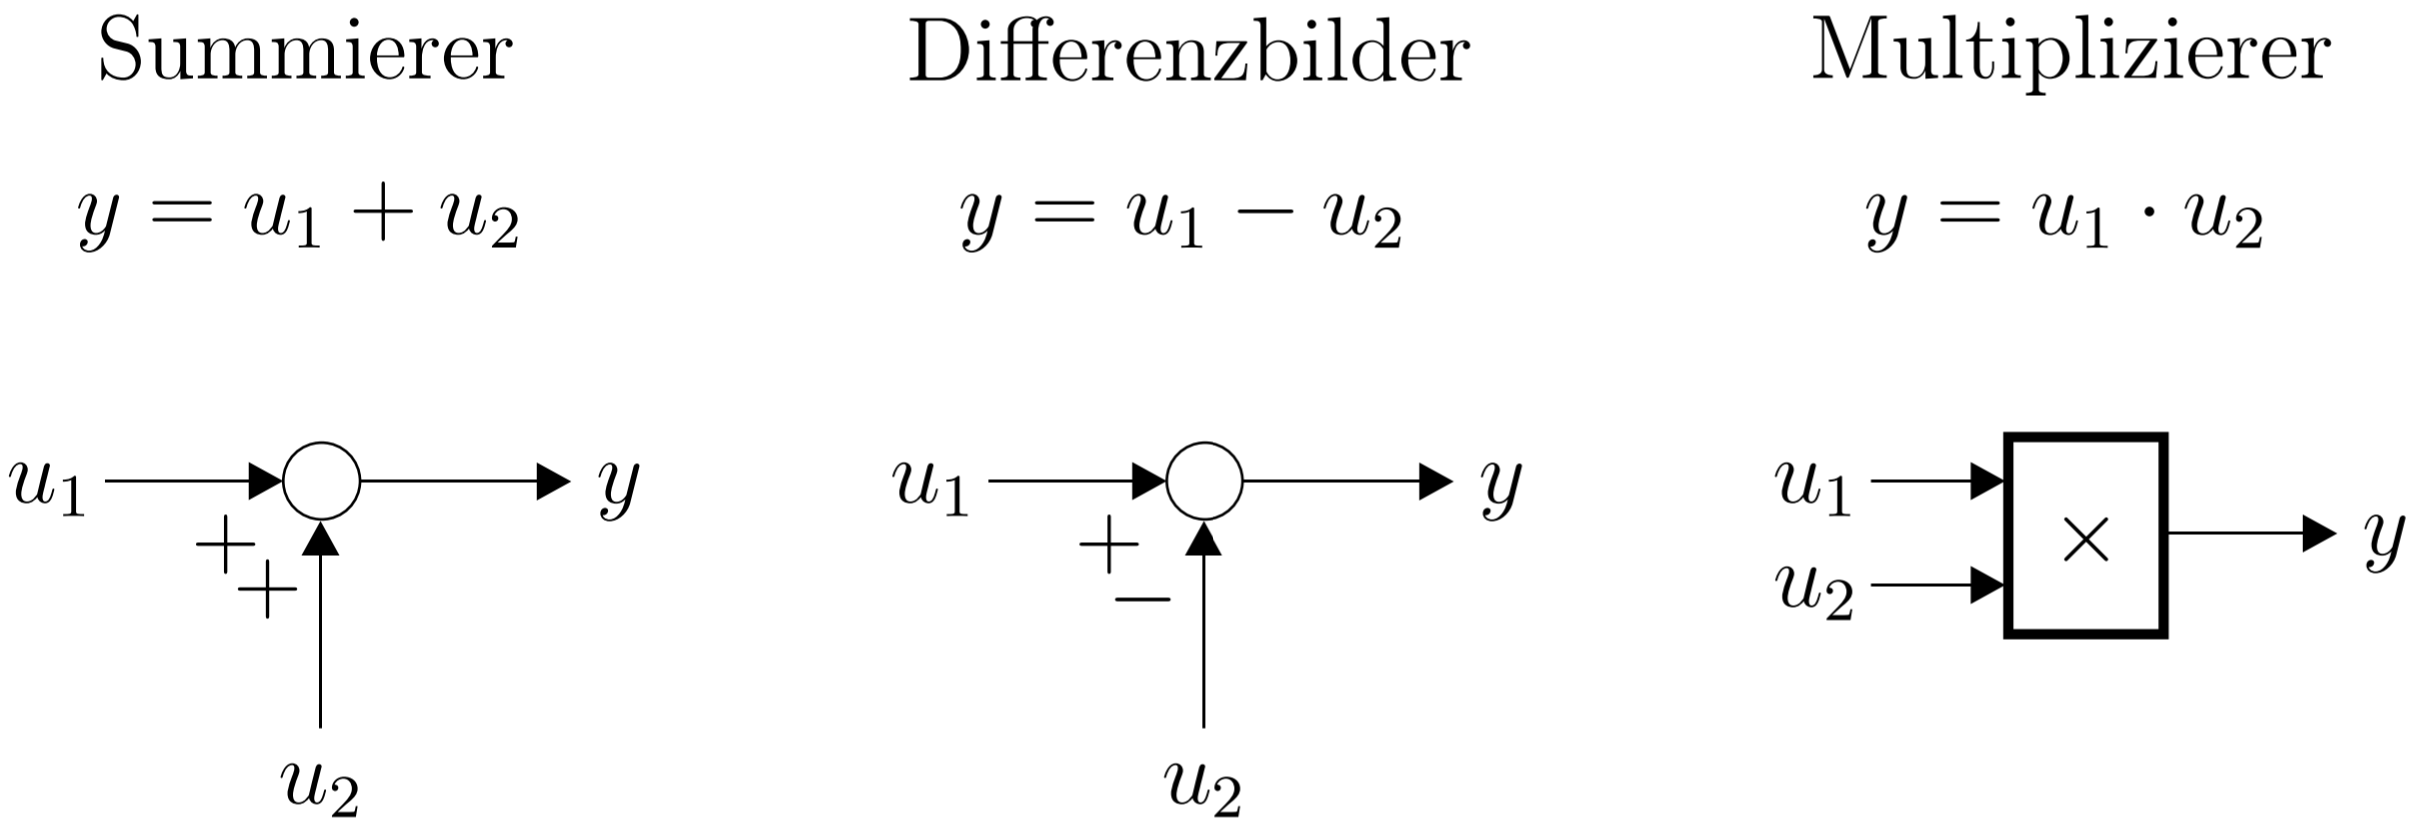
\includegraphics[width=10 cm]{./bilder/grundglieder/statischeGlieder.png} \\
	
	\subsection{dynamische Glieder \skript{25-41, 202-206}}
		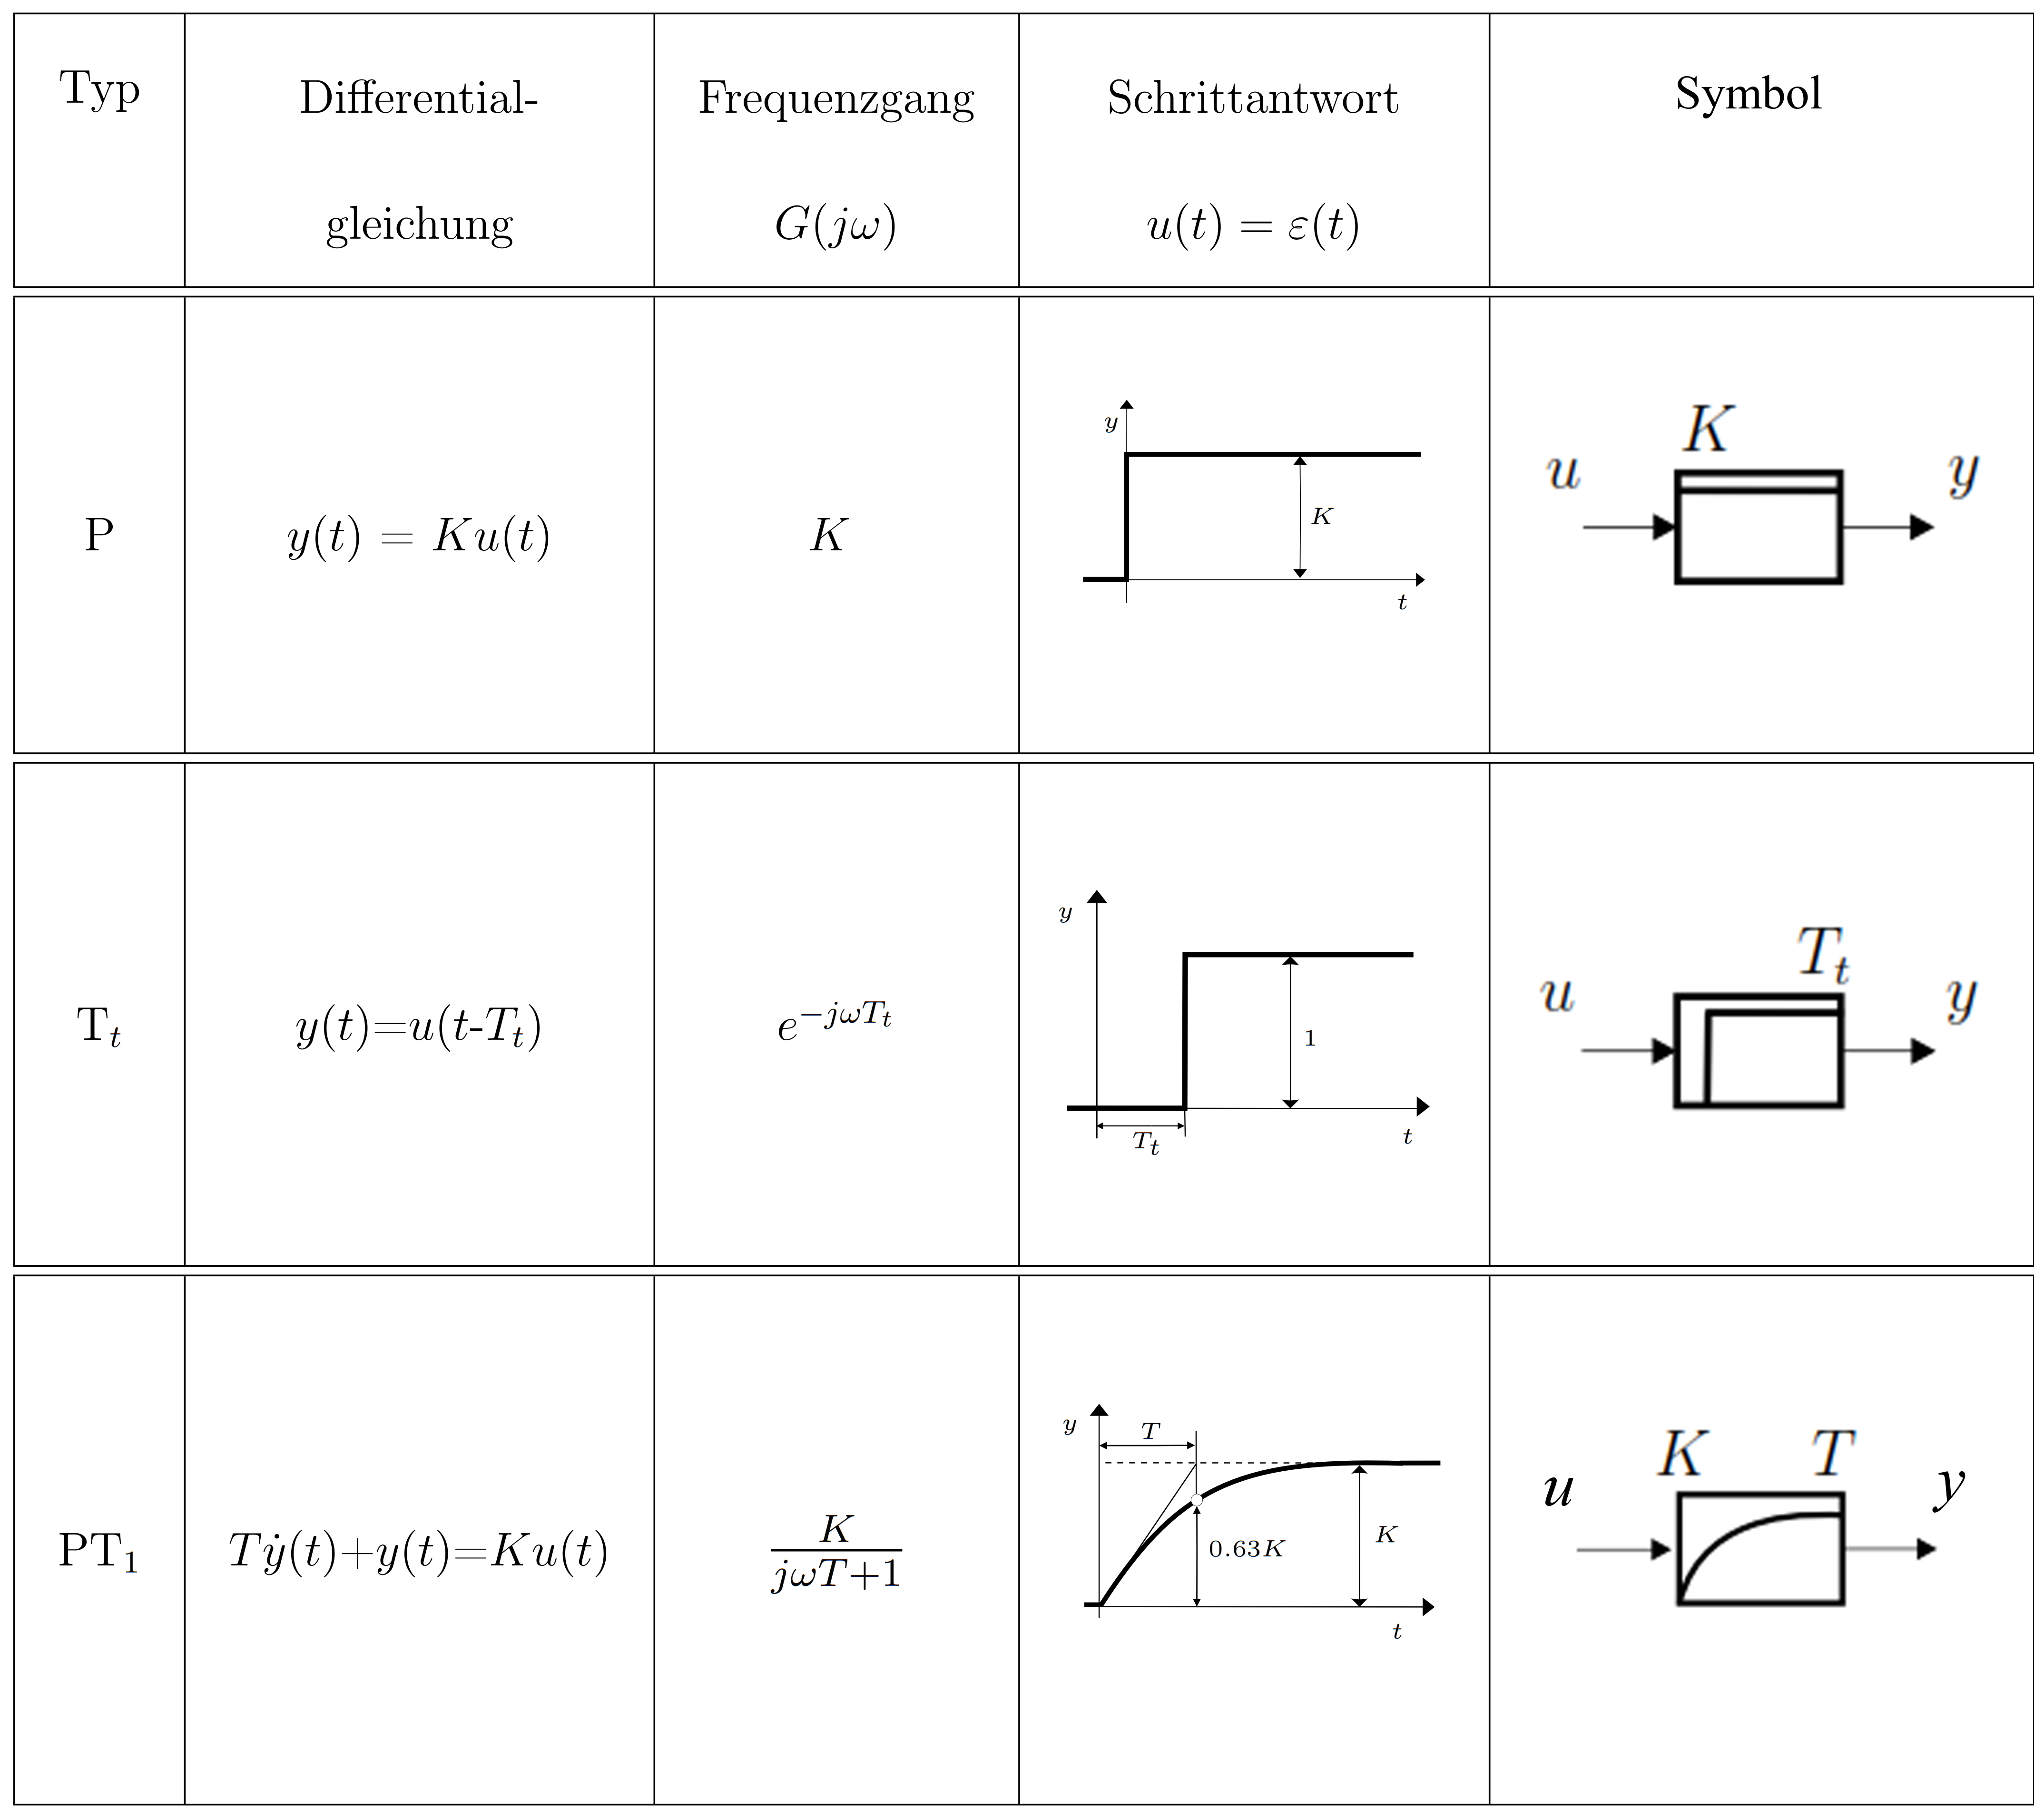
\includegraphics[width=13.5 cm]{./bilder/grundglieder/glieder1.png} \\
		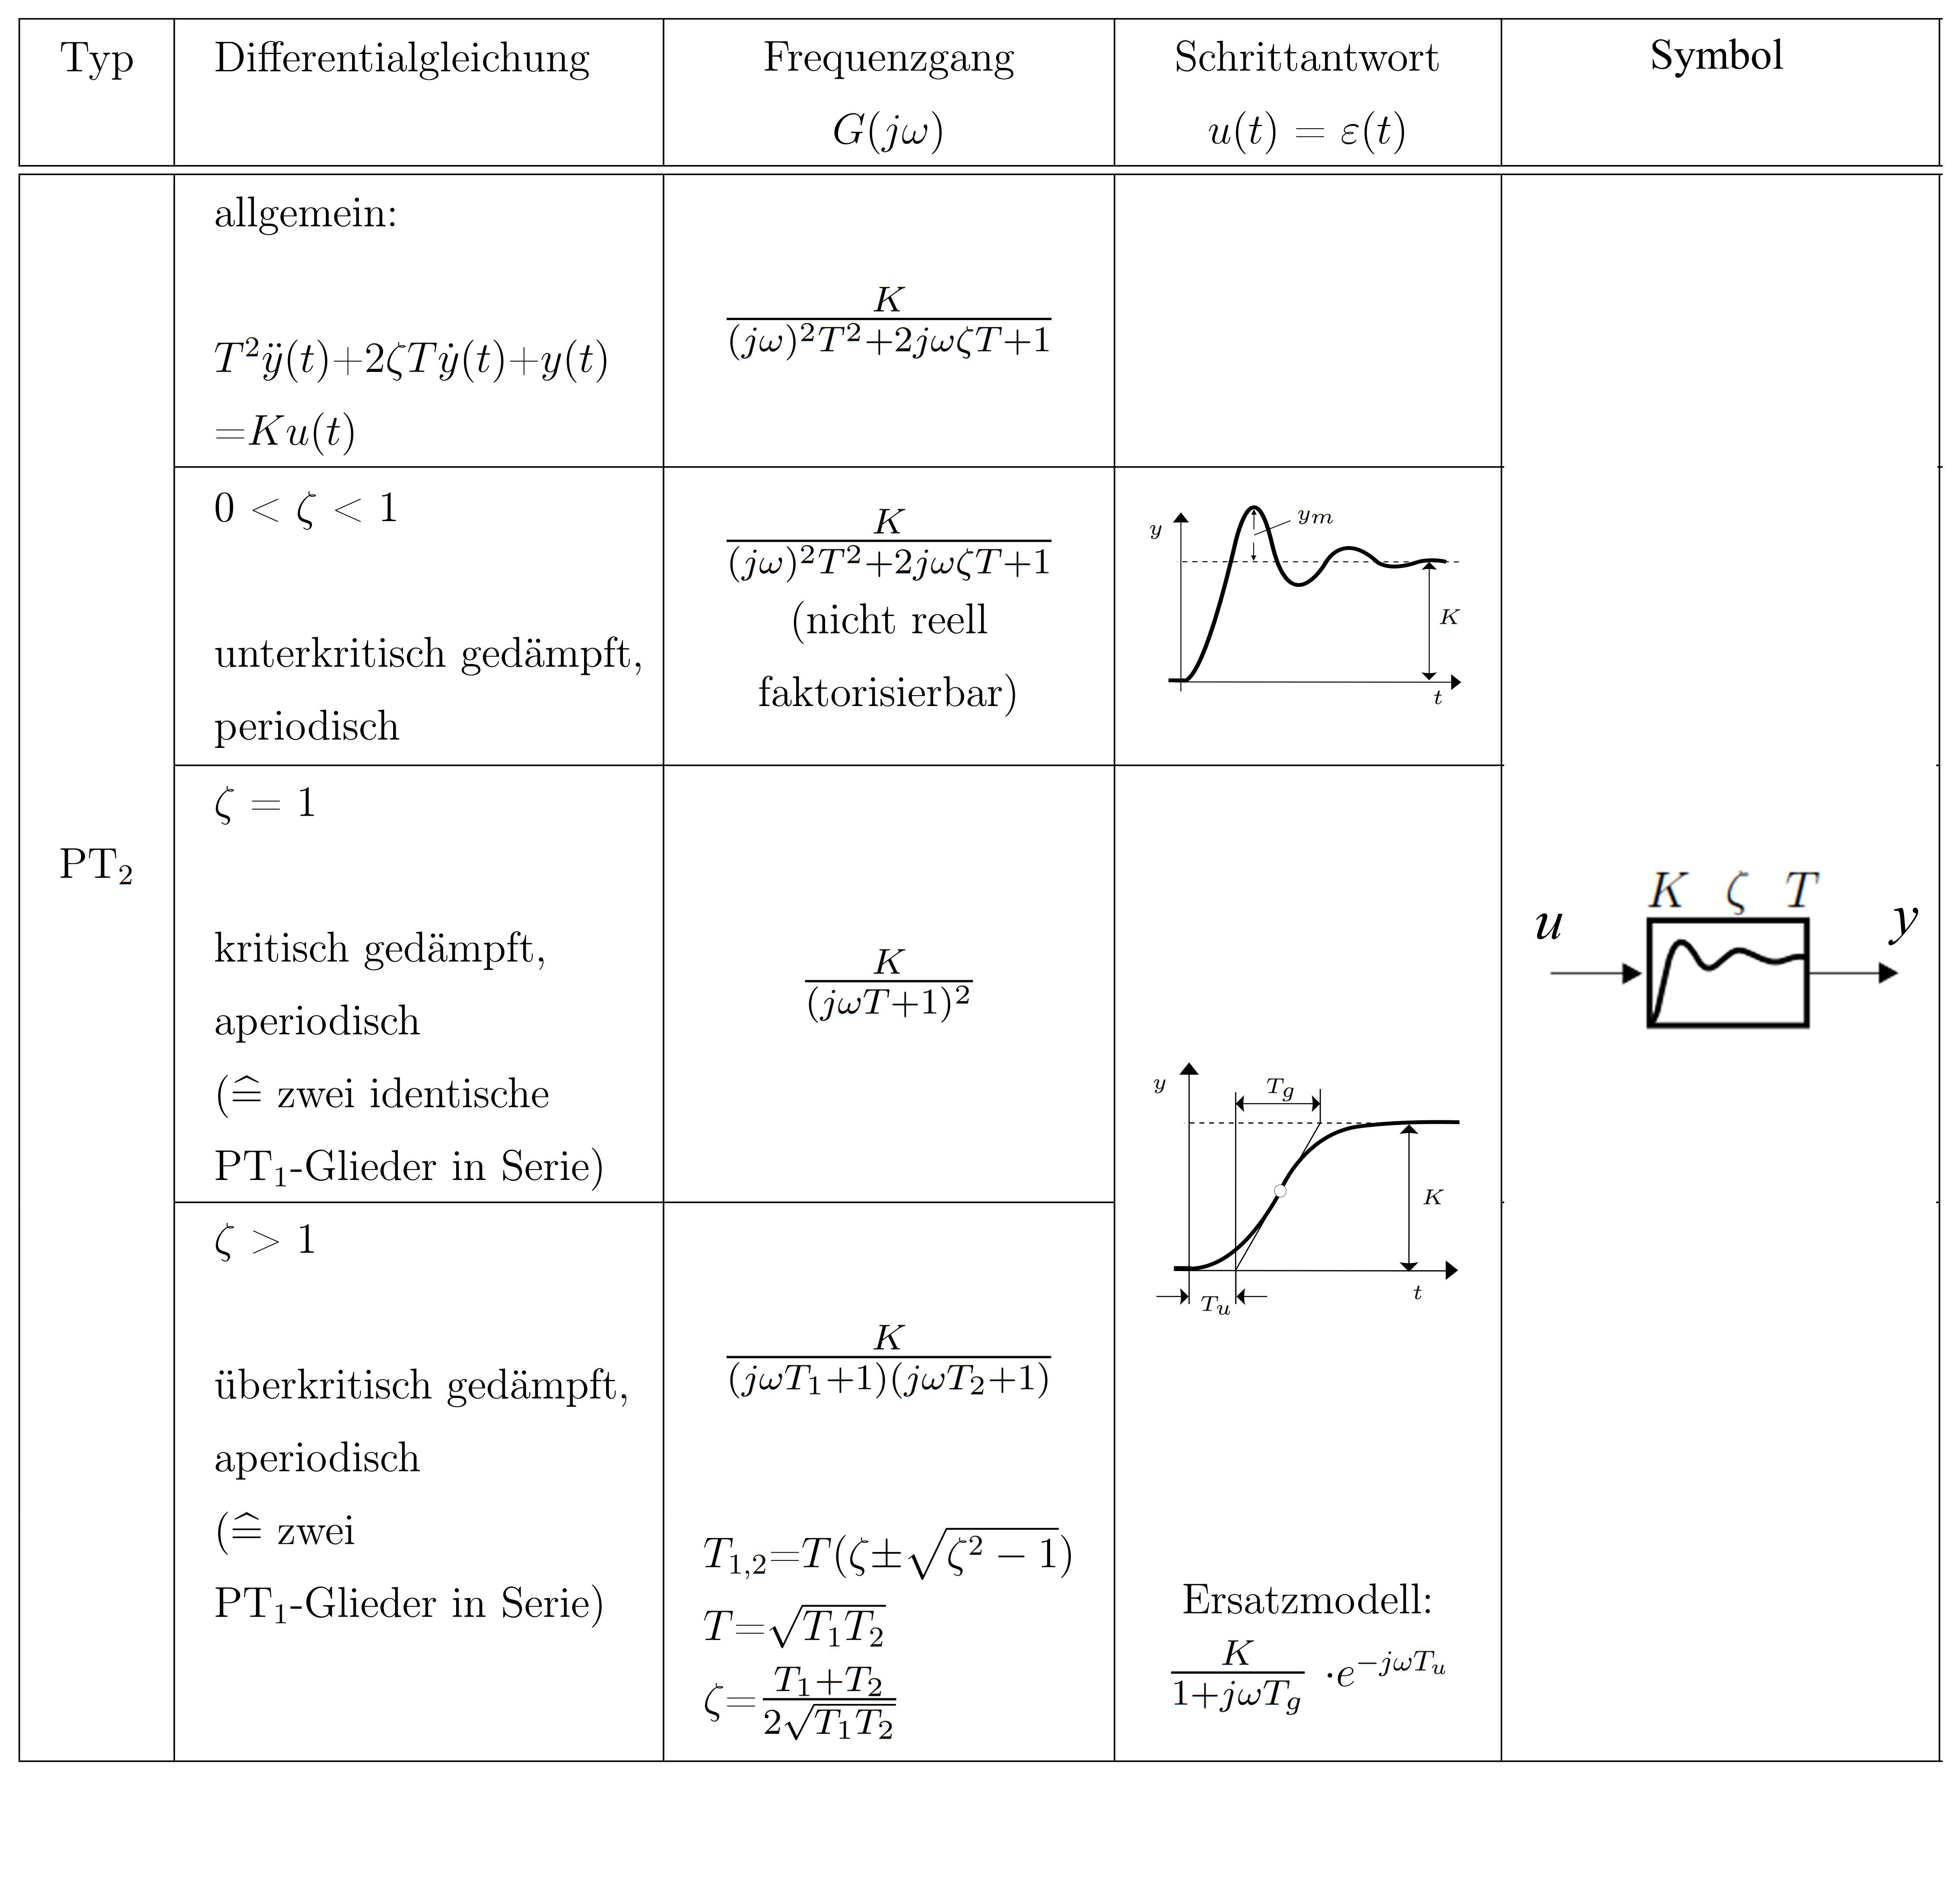
\includegraphics[width=13.5 cm]{./bilder/grundglieder/glieder2.png} \\
		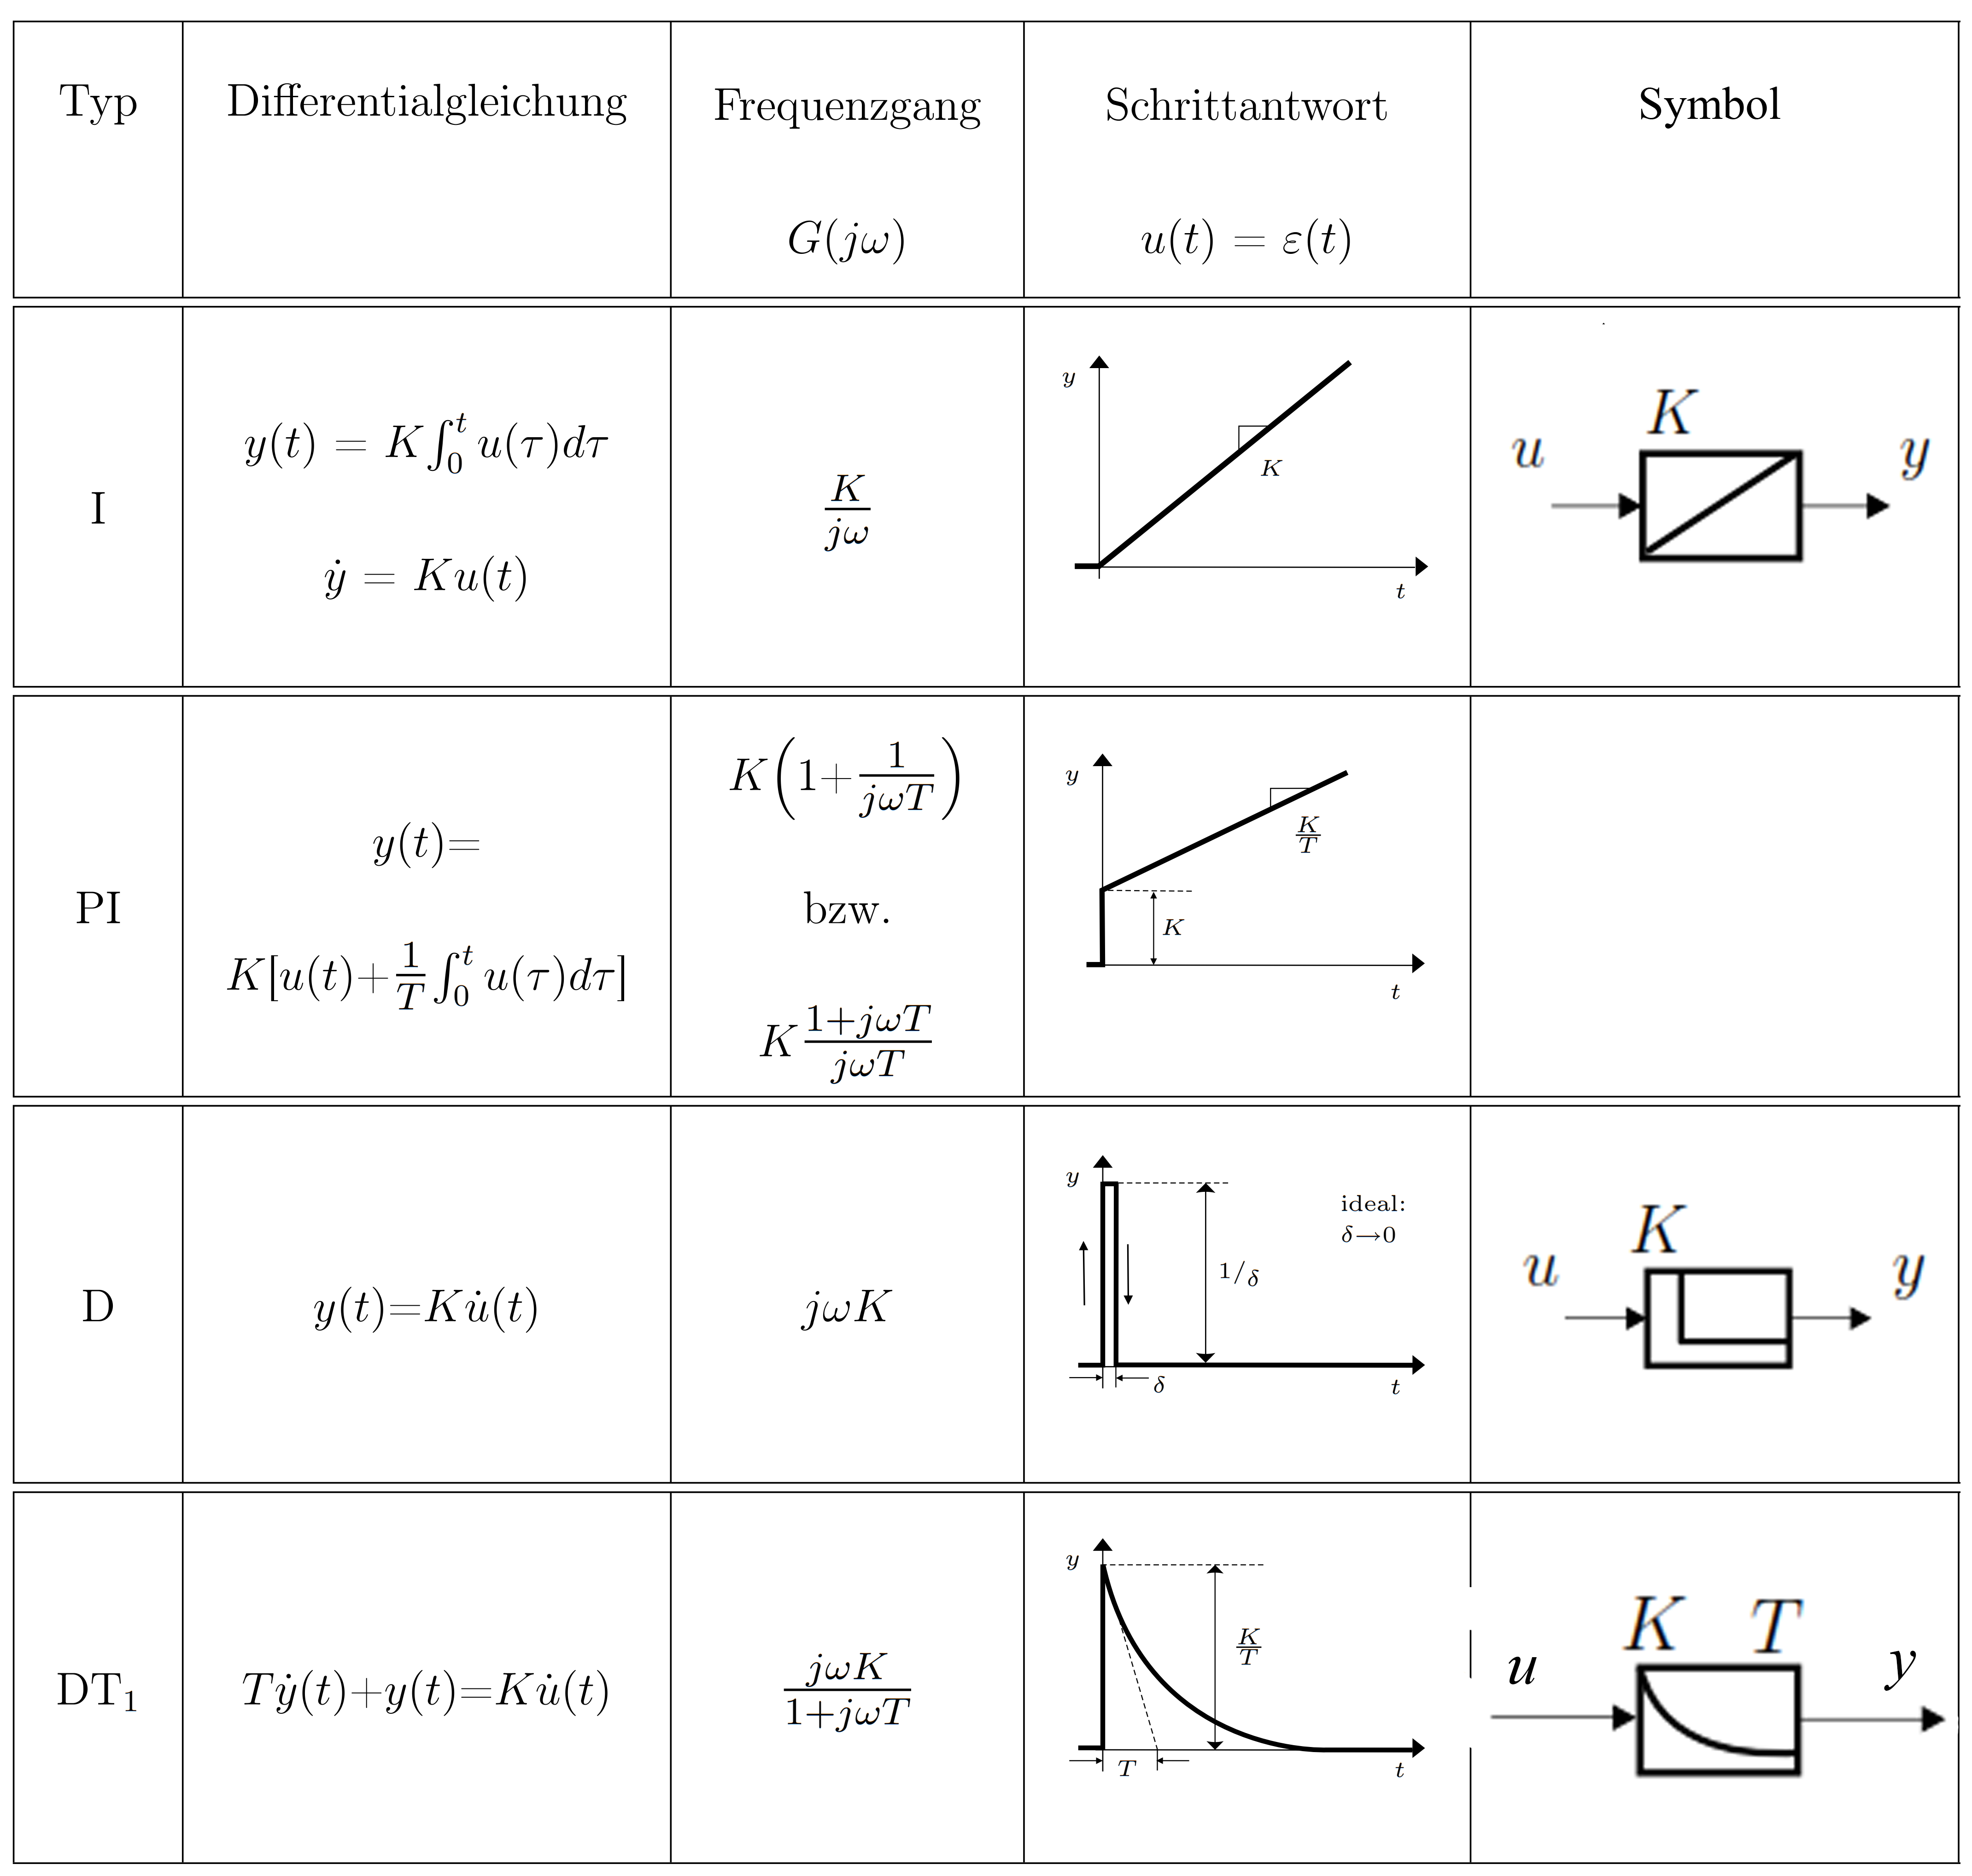
\includegraphics[width=13.5 cm]{./bilder/grundglieder/glieder3.png} \\
		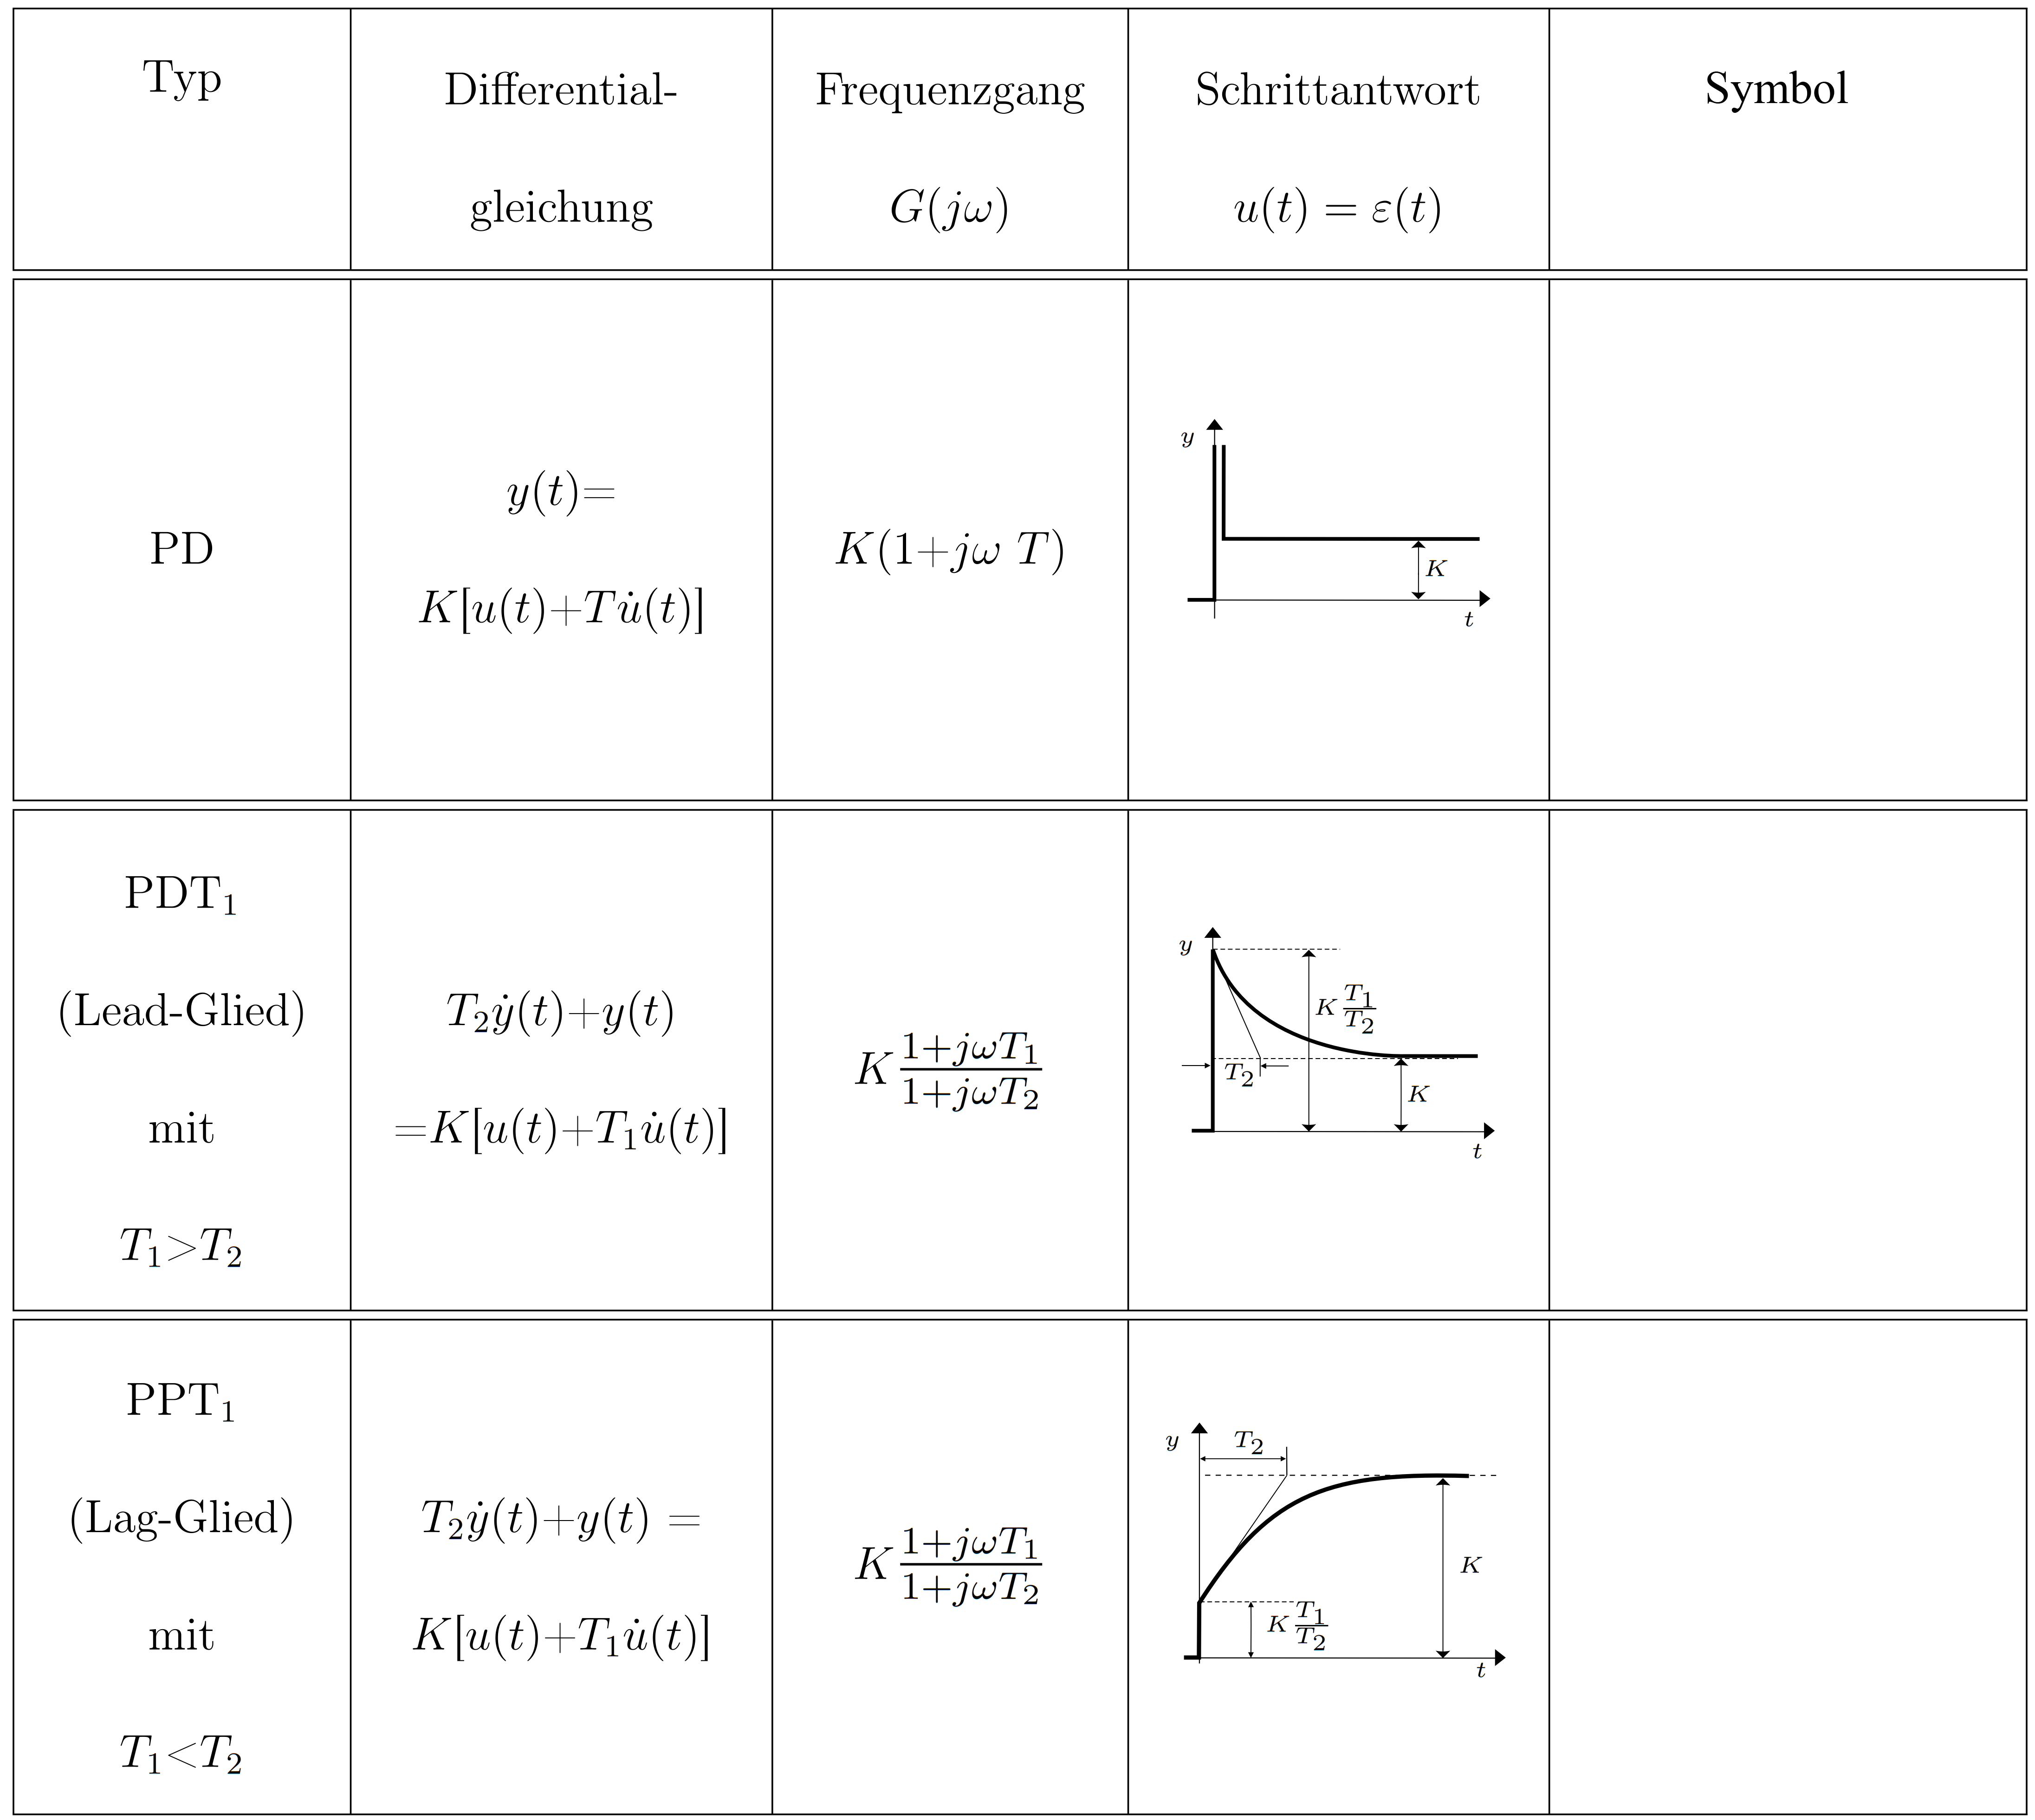
\includegraphics[width=13.5 cm]{./bilder/grundglieder/glieder4.png} \\
		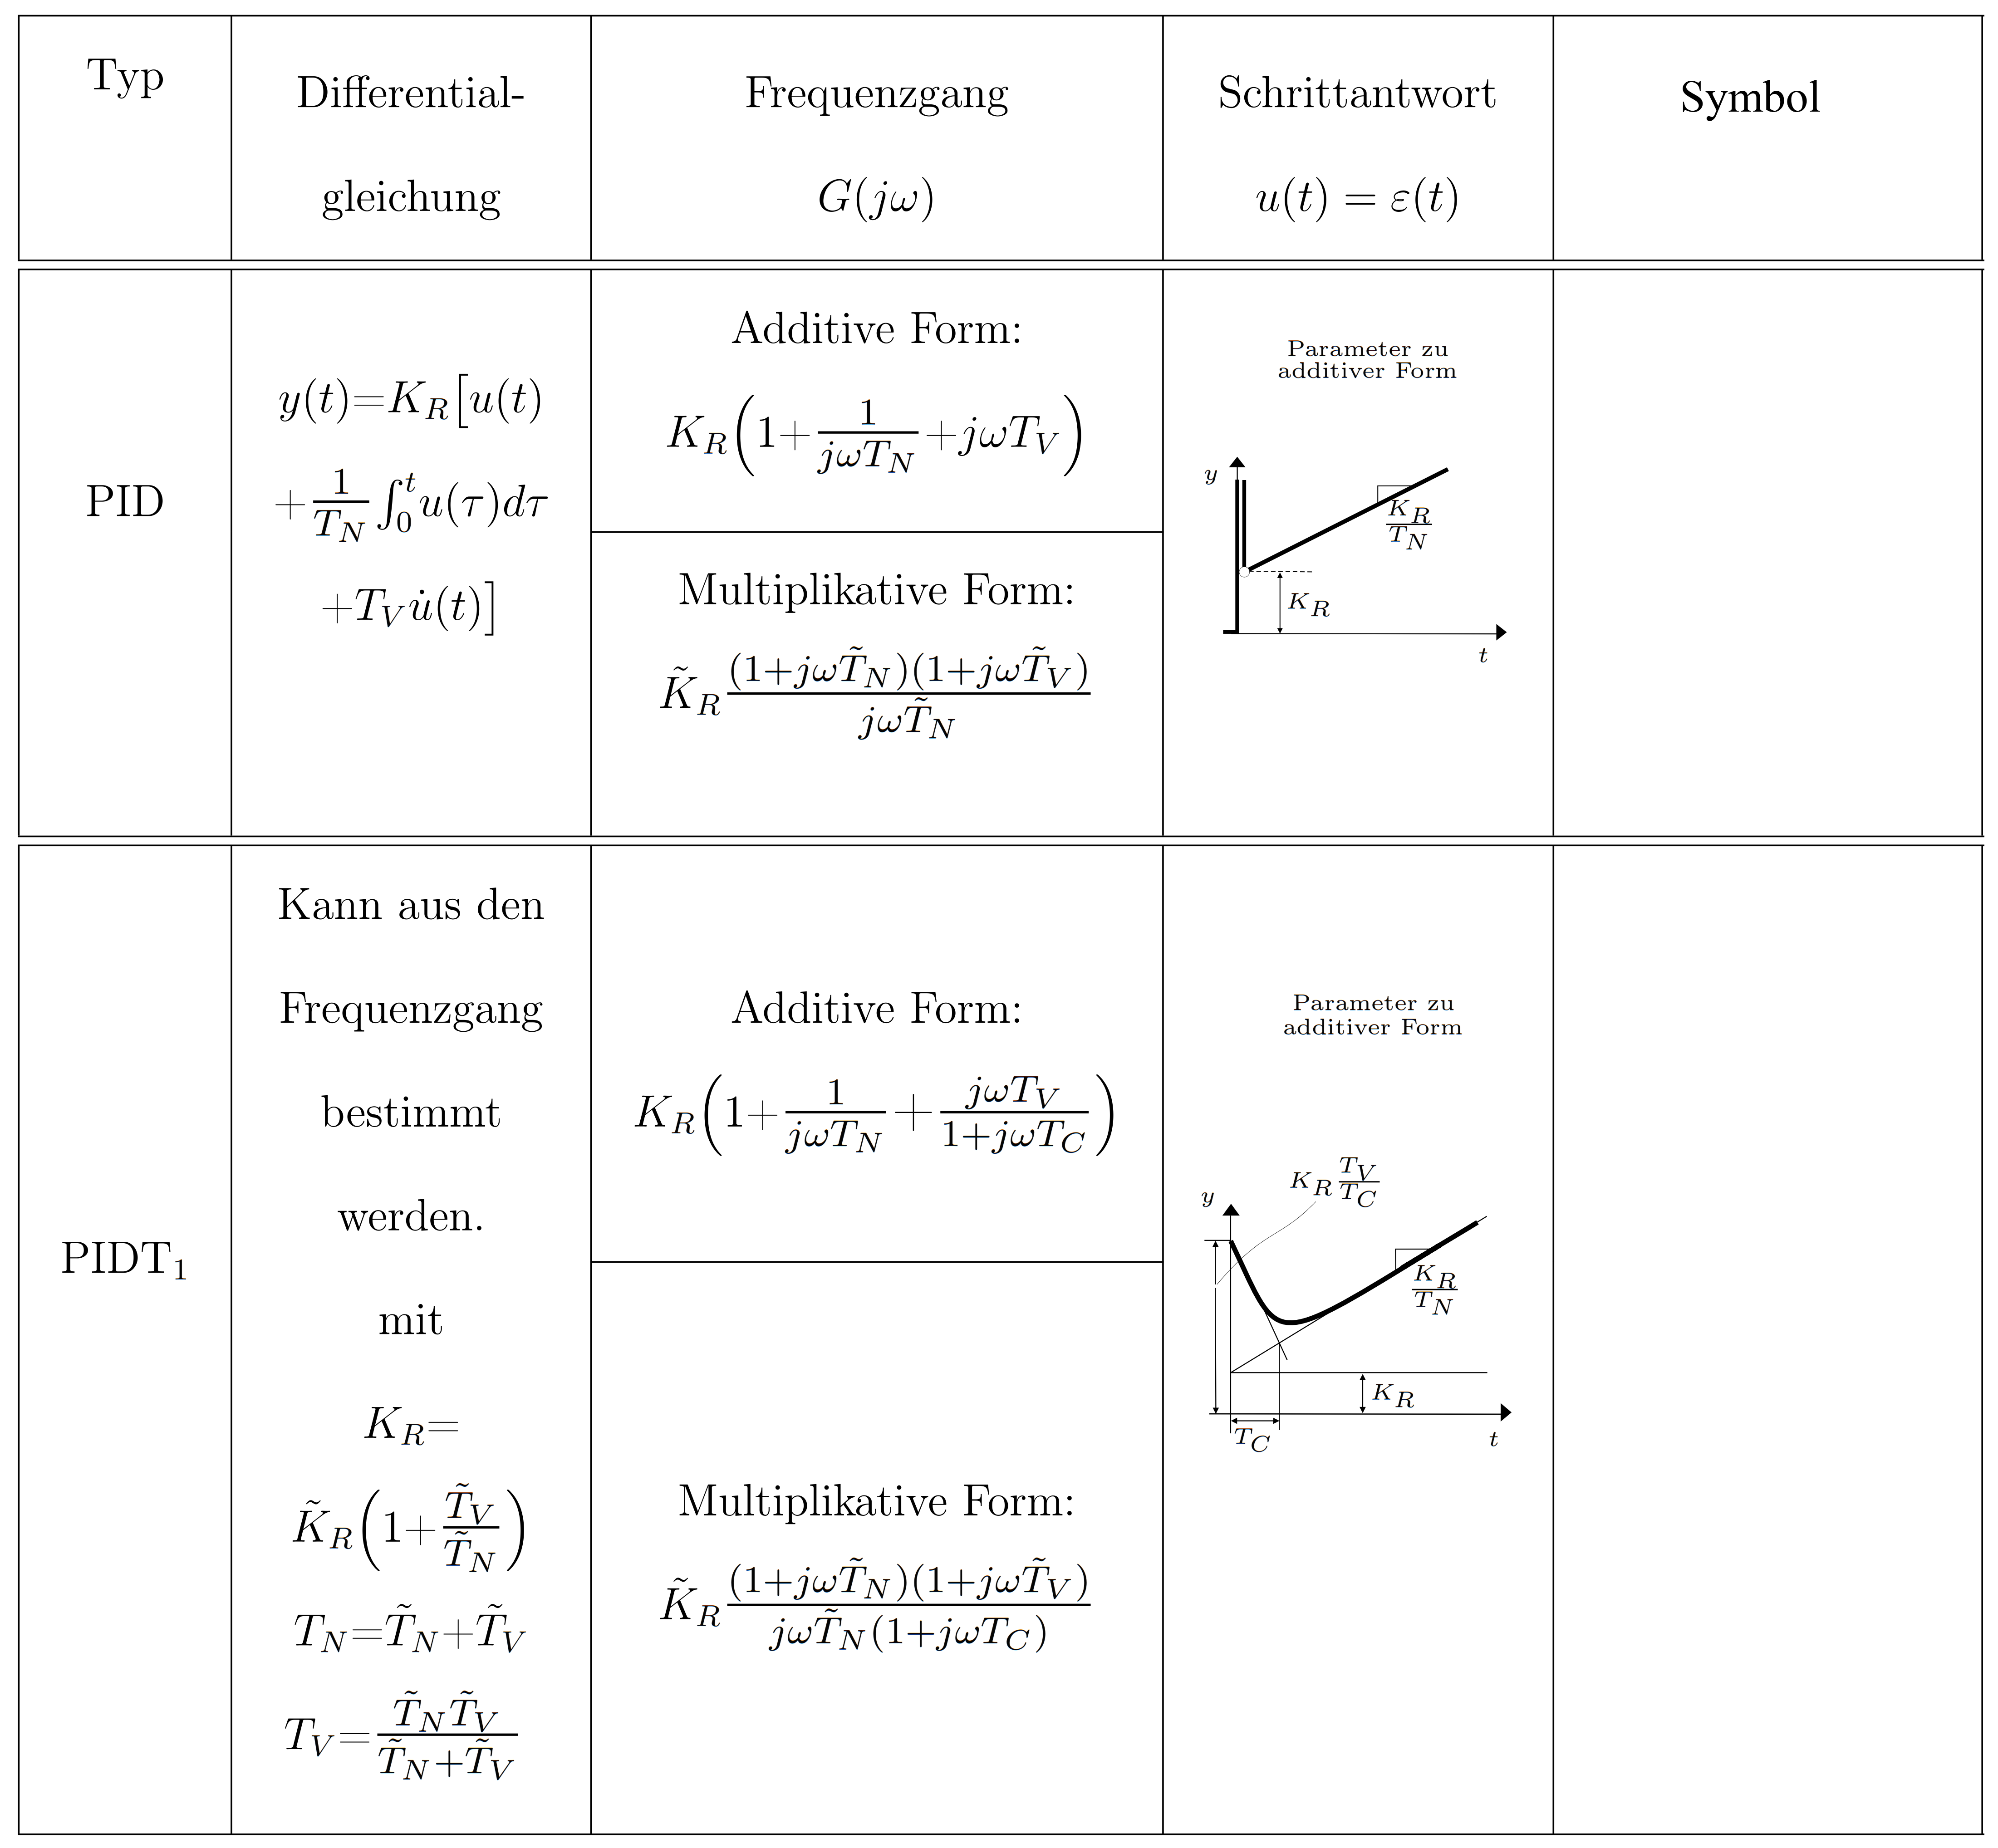
\includegraphics[width=13.5 cm]{./bilder/grundglieder/glieder5.png} \\

%\vspace{0.5cm}
%\rotatebox{90}{
%  \begin{minipage}[]{23cm}
%	\begin{tabular}{|l|l|l|l|l|l|}
%    	\hline
%    	\textbf{Benennung}	&\textbf{Funktion}	&\textbf{UTF}	& \textbf{Sprungantw.}	
%    	&\textbf{Verlauf Sprungantw.}	&\textbf{Symbol}\\
%    	\hline
%    	\hline
%    	\textbf{P-Glied} \formelbuch{26} & $y(t)=K u(t)$	& K & K
%    	&\begin{minipage}{2.4cm}
%         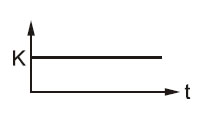
\includegraphics[width=2.4cm,trim=0 0 -5 -5]{./bilder/verlaufP.jpg}
%         \end{minipage}
%    	&\begin{minipage}{2.4cm}
%         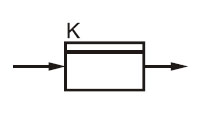
\includegraphics[width=2.4cm]{./bilder/p-Glied.jpg}
%         \end{minipage}\\
%    	\hline
%    	%
%    	\textbf{I-Glied} \formelbuch{29} &
%    	\parbox{3cm}{$\dot{y}= K u(t)$\\
%    				$y=K\int \limits_0^t u(t) dt$\\}
%    				&$\dfrac{K}{s}$ & Kt
%    	&\begin{minipage}{2.4cm}
%         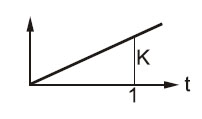
\includegraphics[width=2.4cm,trim=0 0 -5 -5]{./bilder/verlaufI.jpg}
%         \end{minipage}
%    	&\begin{minipage}{2.4cm}
%         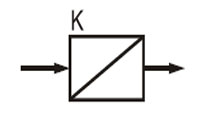
\includegraphics[width=2.4cm]{./bilder/I-Glied.jpg}
%         \end{minipage}\\
%    	\hline	
%    	\textbf{Totzeit-Glied} \formelbuch{30}	
%    	&$y(t)=u(t-T_t)$	&$e^{-T_t s}$	&$K \cdot u(t-T_t)$
%    	&\begin{minipage}{2.4cm}
%         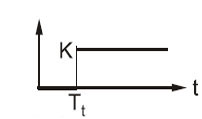
\includegraphics[width=2.4cm,trim=0 0 -5 -5]{./bilder/verlaufTt.jpg}\\
%         \end{minipage}
%    	&\begin{minipage}{2.4cm}
%         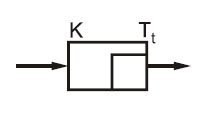
\includegraphics[width=2.4cm]{./bilder/Tt-Glied.jpg}
%         \end{minipage}\\
%		\hline
%    	 \begin{minipage}{4cm}
%			\vspace{0.2cm}
%			\textbf{PT$_1$-Glied} \formelbuch{31}\\
%			%    	   	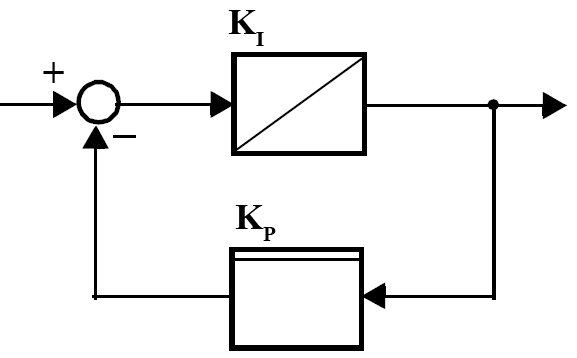
\includegraphics[width=4cm]{./bilder/PT1.png}   
%         \end{minipage}
%		 &\parbox{3cm}{$T\dot{y}+y=K u(t)$\\\\
%		 $T = \dfrac{1}{K_i \cdot K_p}$\\
%		 $K = \dfrac{1}{K_p}$}	 
%		 &$\dfrac{K}{1+Ts}$
%    	 &$K(1-e^{-\frac{t}{T}})$
%    	 &\begin{minipage}{2.4cm}
%         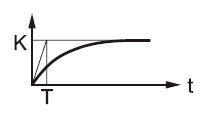
\includegraphics[width=2.3cm]{./bilder/verlaufPT1.jpg}
%         \end{minipage}
%    	&\begin{minipage}{2.4cm}
%         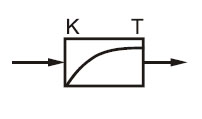
\includegraphics[width=2.3cm]{./bilder/Pt1-Glied.jpg}
%         \end{minipage}\\
%    	\hline
%    	\multicolumn{6}{|l|}{
%    		\parbox{18cm}{\textbf{PT$_1$-Glied mit Grundelementen} ($K$: Verstärkung; $T$: Zeitkonstante):\\
%    				\begin{minipage}{10cm}
%    				    \hspace*{4cm}
%    				    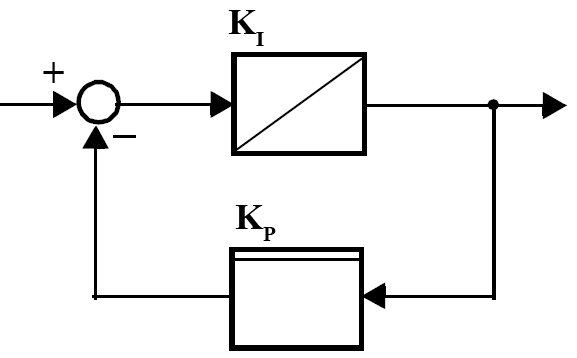
\includegraphics[width=4cm]{./bilder/PT1.png}
%    				\end{minipage}
%    				\begin{minipage}{7cm}
%    					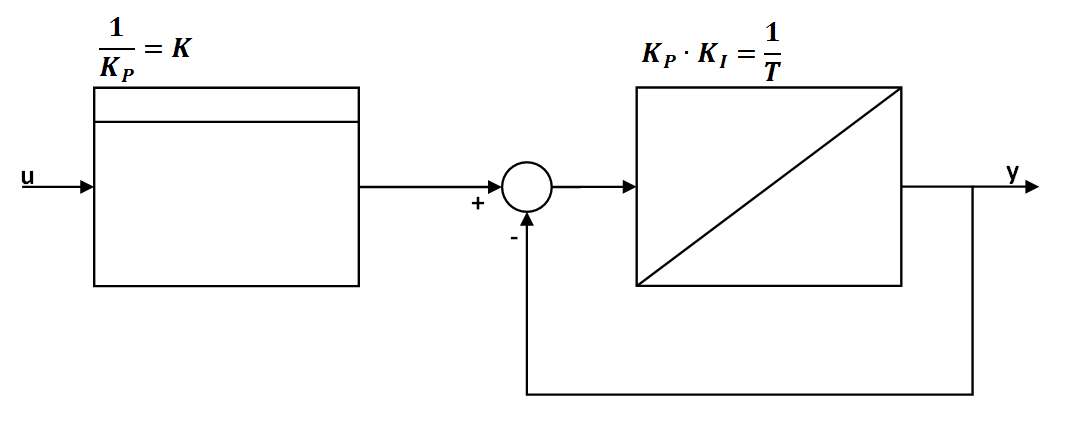
\includegraphics[width=6cm]{./bilder/PT1_2.png}
%    				\end{minipage}
%    		}
%    	}\\
%    	\hline
%		\textbf{PT$_2$-Glied} \formelbuch{34}	
%    	&$T^2\cdot\ddot{y}(t)+2\zeta T\cdot \dot{y}(t)+y(t)=K\cdot u(t)$	
%    	&$\dfrac{K}{1+2dTs+T^2s^2}$	
%    	& siehe unten *
%    	&	\begin{minipage}{1.5 cm}
%         	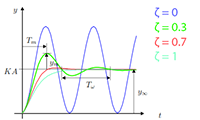
\includegraphics[width=2.2cm,trim=0 0 -3 -5]{./bilder/pt2.png}
%         	\end{minipage}
%         	\begin{minipage}{0.9 cm}
%         	Test
%         	\end{minipage}
%        \hline 
%    	&\begin{minipage}{2.4cm}
%         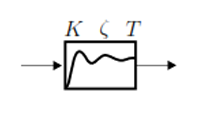
\includegraphics[width=2.4cm]{./bilder/pt2_symbol.png}
%         \end{minipage}\\
%		\hline
%		\textbf{D-Glied} \formelbuch{37}	
%    	&$y(t)= K\cdot \dot{u}(t)$	
%    	&$K \cdot s$	
%    	&$KA \cdot \delta(t)$
%    	&\begin{minipage}{2.4cm}
%         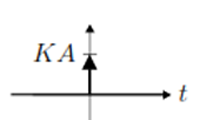
\includegraphics[width=2.2cm,trim=0 0 -3 -5]{./bilder/d-glied.png}\\
%         \end{minipage}
%    	&\begin{minipage}{2.4cm}
%         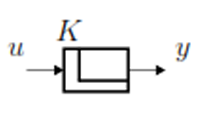
\includegraphics[width=2.4cm]{./bilder/d-glied_symbol.png}
%         \end{minipage}\\
%		\hline
%	\textbf{DT$_1$-Glied} \formelbuch{38}	
%    	&$T\cdot \dot{y}(t)+y(t)= K\cdot \dot{u}(t)$	
%    	&$\frac {K \cdot s} {1+Ts}$	
%    	&$\frac {K\cdot A} {T \cdot e^-\frac {t}{T}}$
%    	&\begin{minipage}{2.4cm}
%         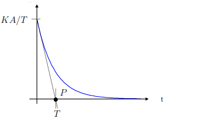
\includegraphics[width=2.2cm,trim=0 0 -3 -5]{./bilder/dt1-glied.png}\\
%         \end{minipage}
%    	&\begin{minipage}{2.4cm}
%         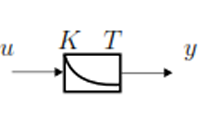
\includegraphics[width=2.4cm]{./bilder/dt1-glied_symbol.png}
%         \end{minipage}\\
%		\hline
%    \end{tabular}
%    \\\\\\   
%         \begin{minipage}[t]{16 cm}
%         * $\left\{\begin{array}{ll}K-\frac{K}{T_1-T_2}\left[T_1e^{-\frac{t}{T_1}}-T_2e^{-\frac{t}{T_2}}\right] & \zeta > 1 (aperiodischer Fall)\\ K-\frac{K}{\sqrt{1-\zeta^2}}e^{-\frac{\zeta}{T}t}\cdot \sin \left[\frac{\sqrt{1-\zeta^2}}{T}t+\arctan \frac{\sqrt{1-\zeta^2}}{\zeta}\right] & \zeta < 1 (periodischer Fall) \\ K-K\left[1+\frac{t}{T}\right]e^{-\frac{t}{T}} & \zeta = 1 (aperiodischer Grenzfall) \end{array}\right.$ 
%         \end{minipage} 
%         \begin{minipage}[t]{8 cm}
%         mit $T_1,2 = \frac{T}{d\pm \sqrt{d^2-1}}$
%         \end{minipage} 
%   \end{minipage}     
%    } 



    \subsection {Elektronische Schaltungen}
    \begin{minipage}{7cm}
    \textbf{P-Glied (nicht inv. Op-Amp)}\\
    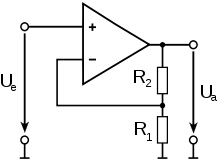
\includegraphics[height=2.5cm]{./bilder/OP-Amp.png} \\
    $K = 1 + \frac{R_2}{R_1}$
    \end{minipage}
    \begin{minipage}{6cm}
	\textbf{P-Glied (inv. Op-Amp)} \\ 
	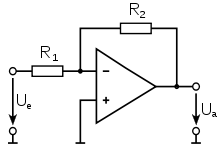
\includegraphics[height=2.5cm]{./bilder/OP-InvAmp.png} \\
	$K=-\frac{R_2}{R_1}$
    \end{minipage}
    \begin{minipage}{6cm}
	\textbf{I-Glied} \\ 
	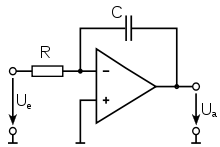
\includegraphics[height=2.5cm]{./bilder/OP-Integrator.png}\\
	$K = - \frac{1}{R \cdot C}$
    \end{minipage}  
    
		